\documentclass[11pt,a4paper]{article}
\usepackage[utf8]{inputenc}
\usepackage[german]{babel}
\usepackage[T1]{fontenc}
\usepackage{amsmath}
\usepackage{amsfonts}
\usepackage{amssymb}
\usepackage{graphicx}
\usepackage[margin=1.25cm]{geometry} % Puts the same margin on all borders of the document

% Packages

\usepackage{hyperref} % Generate hyperlinks to referenced items
\usepackage{adjustbox} % Used to change parameters in \includegraphics[scale=•]{•}
\usepackage{enumitem} % Provides several options for lists
\usepackage{verbatim} % Package to use \begin{comment}
\usepackage{pdfpages} % Used to import PDF pages
\usepackage{multirow} % Allows us to have a single cell in a table span multiple rows
\usepackage{makecell} % Allows us to format multiple lines in a single cell
\usepackage{minted} % Used to syntax highlight code
\usepackage{xcolor}  % Gives access to coloring text
\usepackage{longtable} % Allows us to create a table over multiple pages
\usepackage{float} % Improved placement of floating items
\usepackage{pdfpages} % Used to import pdf pages
\usepackage{booktabs} % Used for horizontal lines instead of \hline



% Settings

\graphicspath{{./files/}} % Sets path for files to the files folder in the same directory

\hypersetup{
    colorlinks=false, %set true if you want colored links
    linktoc=all,     %set to all if you want both sections and subsections linked
    linkcolor=blue,  %choose some color if you want links to stand out
}


\begin{titlepage}
  \title{Rechnerorganisation} % document_name-type_of_document
  \author{Jonas Milkovits}
  \date{Last Edited: \today}
\end{titlepage}

\begin{document}

\pagenumbering{gobble}
\maketitle
\pagenumbering{roman} % i, ii, iii on beginning pages, that don't have content
\tableofcontents
\clearpage
\pagenumbering{arabic} % 1,2,3 on content pages

\section{Einführung}

\subsection{Begrifflichkeiten und Grundlagen}
    \begin{itemize}
        \item \textbf{Abstraktion}
            \begin{itemize}
                \item Wichtiges und zentrales Konzept der Informatik
                \item Verstecken unnötiger Details (für spezielle Aufgabe unnötig)
            \end{itemize}
        
        \item \textbf{Schichtenmodell}
        \item[]
            \begin{minipage}{0.3\textwidth}
            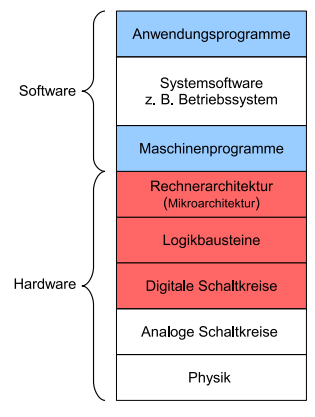
\includegraphics[width=5cm]{schichtenmodell.PNG}
            \end{minipage}
            \begin{minipage}[t]{0.6\textwidth}
            \vspace{-3cm}
                \begin{itemize}
                    \item Untere Schicht erbringt Dienstleistungen für höhere Schicht
                    \item Obere Schicht nutzt Dienste der niedrigeren Schicht
                    \item Eindeutige Schnittstellen zwischen den Schichten
                    \item Vorteile:
                        \begin{itemize}
                            \item Austauschbarkeit einzelner Schichten
                            \item Nur Kenntnis der bearbeitenden Schicht notwendig
                        \end{itemize}
                    \item Nachteile:
                        \begin{itemize}
                            \item ggf. geringere Leistungsfähigkeit des Systems
                        \end{itemize}
                \end{itemize}
            \end{minipage}
        
        \item \textbf{Grundbegriffe}
            \begin{itemize}
                \item Computer:
                    \begin{itemize}
                        \item Datenverarbeitungssystem
                        \item Funktionseinheit zur Verarbeitung und Aufbewahrung von Daten
                        \item Auch Rechner, Informationsverarbeitungssystem, Rechnersystem,..
                        \item Steuerung eines Rechnersystems folgt über ladbares Programm (Maschinenbefehle)
                    \end{itemize}
                \item Grundfunktionen, die ein Rechner ausführt
                    \begin{itemize}
                        \item Verarbeitung von Daten (Rechnen, logische Verknüpfungen,..)
                        \item Speichern von Daten (Ablegen, Wiederauffinden, Löschen)
                        \item Umformen von Daten (Sortieren, Packen, Entpacken)
                        \item Kommunizieren (Mit Benutzer, mit anderen Rechnersystemen)
                    \end{itemize}
            \end{itemize}

        \item \textbf{Komponenten eines Rechnersystems}
            \begin{itemize}
                \item Prozessor
                    \begin{itemize}
                        \item Zentraleinheit, Central Processing Unit (CPU)
                        \item Ausführung von Programmen
                    \end{itemize}
                \item Speicher
                    \begin{itemize}
                        \item Enthält Programme und Daten (Speichersystem)
                    \end{itemize}
                \item Kommunikation
                    \begin{itemize}
                        \item Transfer von Informationen zwischen Speicher und Prozessor
                        \item Kommunikation mit der Außenwelt (Ein-/Ausgabesystem)
                    \end{itemize}
                \item[] 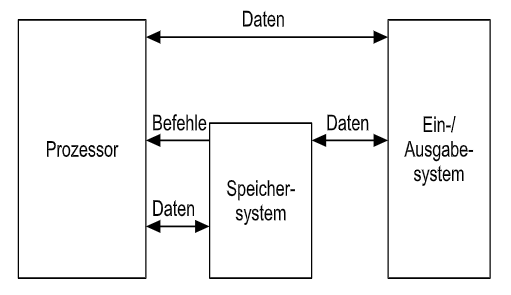
\includegraphics[width=8cm]{rechnersystem.PNG}
            \end{itemize}

        \item \textbf{Nähere Informationen zum Speicher} 
            \begin{itemize}
                \item Explizite Nutzung des Speichersystem
                    \begin{itemize}
                        \item Internet Prozessorspeicher/Register
                            \begin{itemize}
                                \item schnelle Register zur temporären Speicherung von Daten/Befehlen
                                \item direkter Zugriff durch Maschinenbefehle
                                \item Technologie: Halbleiter ICs
                            \end{itemize}
                        
                        \item Hauptspeicher
                            \begin{itemize}
                                \item relativ großer und schneller Speicher für Programme/Daten 
                                \item direkter Zugriff durch Maschinenbefehle 
                                \item Technologie: Halbleiter ICs
                            \end{itemize}

                        \item Sekundärspeicher
                            \begin{itemize}
                                \item großer, aber langsamer Speicher für permanente Speicherung
                                \item indirekter Zugriff über E/A-Programme (Daten $\rightarrow$ Hauptspeicher)
                                \item Technologie: Halbleiter ICs, Magnetplatten, optische Laufwerke
                                \item z.B.: Festplatte
                            \end{itemize}
                    \end{itemize}

                \item Implizite (transparente) Nutzung 
                    \begin{itemize}
                        \item Für das Maschinenprogramm transparent
                        \item bestimmte Register auf dem Prozessor 
                        \item Cache-Speicher
                    \end{itemize}
                
                \item[] 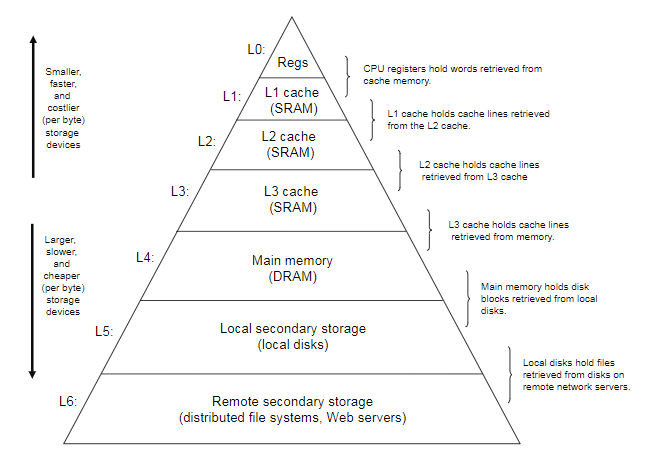
\includegraphics[width=12cm]{speicherhierarchie}
                
                \item Speicherorganisation: Big-Endian und Little-Endian 
                \item[]
                    \begin{minipage}{0.2\textwidth}
                    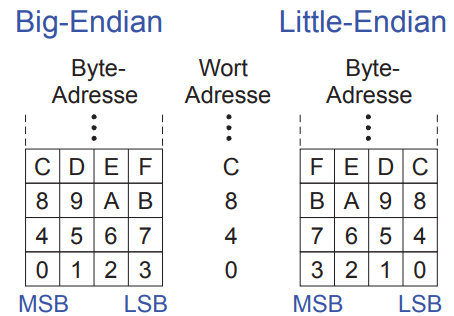
\includegraphics[width=4cm]{bigLittleEndian.PNG}
                    \end{minipage}
                    \begin{minipage}[t]{0.7\textwidth}
                    \vspace{-1.2cm}
                        \begin{itemize}
                            \item Schemata für Nummerierung von Bytes in einem Wort
                            \item Big-Endian: Bytes werden vom höchstwertigen Ende gezählt
                            \item Little-Endian: Bytes werden vom niederstwertigen Ende gezählt
                        \end{itemize}
                    \end{minipage}
            \end{itemize}
            
    \end{itemize}

\subsection{Streifzug durch die Geschichte}

    \begin{itemize}
        \item \textbf{Übersicht über die geschichtliche Entwicklung mit wichtigsten Meilensteinen}
        \begin{itemize}
            \item[] 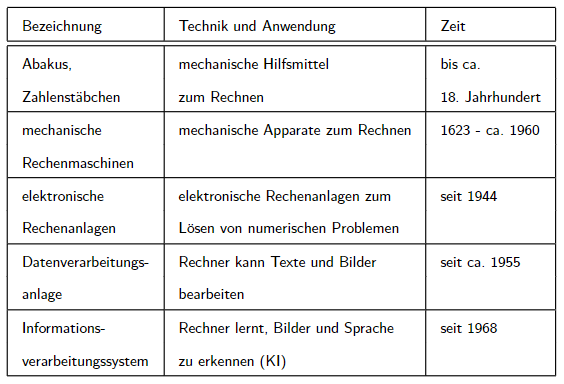
\includegraphics[width=12cm]{geschichtsTabelle1.PNG}
        \end{itemize}
        
        \item \textbf{Fünf Rechnergenerationen im Überblick:}
            \begin{itemize}
                \item[] 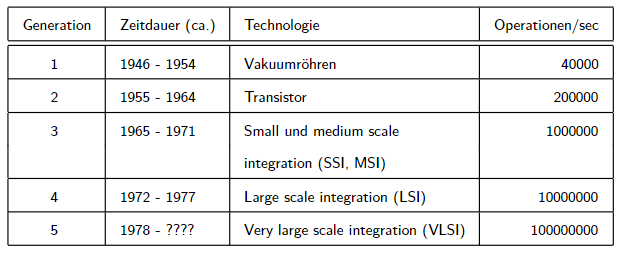
\includegraphics[width=12cm]{rechnergenerationen} 
            \end{itemize}
        
        \item \textbf{Rechner im elektronischen Zeitalter}
            \begin{itemize}
                \item 1954: Entwicklung der Programmiersprache Fortran
                \item 1955: Erster Transistorrechner
                \item 1957: Entwicklung Magnetplattenspeicher, Erste Betriebssysteme für Großrechner
                \item 1968: Erster Taschenrechner
                \item 1971: Erster Mikroprozessor
                \item 1981: Erster IBM PC, Beginn des PC-Zeitalters
            \end{itemize}
    \end{itemize}

\subsection{Ethik in der Informatik}

    \begin{itemize}
        \item Ethik in der Informatik
            \begin{itemize}
                \item Ethik: Bewertung menschlichen Handelns
                \item Verbindung zur Informatik: Anwendung von Rechnern für kriegisches Handelns
                \item \textbf{Dual-Use-Problematik}: Verwendbarkeit von Rechnern für zivile als auch militärische Zwecke
            \end{itemize}
        
        \item Digitale Souveränität
            \begin{itemize}
                \item Souveränität: Fähigkeit zur Selbstbestimmung (Eigenständigkeit, Unabhängigkeit)
                \item Digitale Souveränität: Souveränität im digitalen Raum
            \end{itemize}
    \end{itemize}

\section{Einführung in die maschinennahe Programmierung}

\subsection{Begrifflichkeiten und Grundlagen}
    \begin{itemize}
        \item \textbf{Allgemein}
            \begin{itemize}
                \item Architektur / Programmiermodell
                    \begin{itemize}
                        \item Programmierersicht auf Rechnersystem 
                        \item Definiert durch Maschinenbefehle und Operanden
                    \end{itemize}
                \item Mikroarchitektur
                    \begin{itemize}
                        \item Hardware-Implementierung der Architektur
                    \end{itemize}
            \end{itemize}
        
        \item \textbf{Programmierparadigmen}
            \begin{itemize}
                \item Synonyme: Denkmuster, Musterbeispiel
                \item Bezeichnet in der Informatik ein übergeordnetes Prinzip
                \item Dieses Prinzip ist für eine ganze Teildisziplin typisch
                \item Manifestiert sich an Beispielen, keine konkrete Formulierung
                \item Maschinensprache (Assembler) ist ein primitives Paradigma              
            \end{itemize}

        \item \textbf{Programmiermodell}
            \begin{itemize}
                \item Bei höheren Programmiersprachen:
                    \begin{itemize}
                        \item Grundlegende Eigenschaften einer Programmiersprache 
                    \end{itemize} 
                \item Bei maschinennaher Programmierung:
                    \begin{itemize}
                        \item Bezeichnet dort den \textbf{Registersatz} eines Prozessors 
                        \item Registersatz besteht aus:
                            \begin{itemize}
                                \item Register, die durch Programme angesprochen werden können
                                \item Liste aller verfügbaren Befehle (\textbf{Befehlssatz})
                            \end{itemize}
                        \item Register, die prozessorintern verwendet werden (IP/PC) zählen nicht zum Registersatz
                            \begin{itemize}
                                \item IC: Instruction Pointer 
                                \item PC: Program Counter
                            \end{itemize}
                    \end{itemize}
            \end{itemize}

        \item \textbf{Verfeinerung des Rechensystems}
            \begin{itemize}
                \item[] 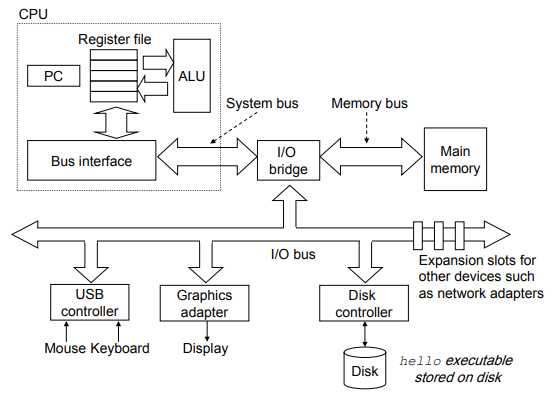
\includegraphics[width=9cm]{modernesRechnersystem.PNG}
                \item {\makebox[6cm][l]{CPU/Prozessor:}} führt die im Hauptspeicher abgelegten Befehle aus 
                \item {\makebox[6cm][l]{ALU/Arithmethic Logical Unit:}} Ausführung der Operationen
                \item {\makebox[6cm][l]{PC/Program Counter:}} Verweis auf nächsten Maschinenbefehl im Hauptspeicher
                \item {\makebox[6cm][l]{Register:}} Schneller Speicher für Operanden
                \item {\makebox[6cm][l]{Hauptspeicher:}} Speichert Befehle und Daten 
                \item {\makebox[6cm][l]{Bus Interface:}} Verbinden der einzelnen Komponenten
            \end{itemize}

        \item \textbf{Assembler}
            \begin{itemize}
                \item Programmieren in der Sprache des Computers
                    \begin{itemize}
                        \item {\makebox[3cm][l]{Maschinenbefehle:}} Einzelnes Wort
                        \item {\makebox[3cm][l]{Befehlssatz:}} Gesamtes Vokabular
                    \end{itemize}
                \item Befehle geben Art der Operation und ihre Operanden an 
                \item Zwei Darstellungen:
                    \begin{itemize}
                        \item Assemblersprache: Für Menschen lesbare Schreibweise für Instruktionen
                        \item Maschinensprache: maschinenlesbares Format (1 und 0)
                    \end{itemize}
            \end{itemize}
        
        \item \textbf{ARM-Architektur - Hier verwendetes Rechnersystem}
            \begin{itemize}
                \item z.B. verwendet bei Raspberry Pi 
                \item ARM: Acorn RISC Machines / Advanced RISC Machines 
                \item Große Verbreitung heutzutage in Smartphones
            \end{itemize}

    \end{itemize}

\pagebreak

\subsection{Phasen der Übersetzung}

        \begin{itemize}
            \item Beispielhaftes \texttt{C}-Programm:
            \item[]
                \begin{minted}[autogobble]{c}
                #include<stdio.h> /* Standard Input/Output */ /* Header-Datei*/
                int main() {
                printf("Hello World\n");
                return 0;
                }
                \end{minted}
            \item \texttt{C}-Programm an sich für den Menschen verständlich
            \item Übersetzung in Maschinenbefehle für Ausführung auf dem Rechnersystem:
            \item[] \includegraphics[width=12cm]{übersetzungsPhasen.PNG}
            \item 1. Phase \textbf{(Preprocessor)}
                \begin{itemize}
                    \item Aufbereitung durch Ausführung von Direktiven (Code mit \#)
                    \item z.B.: Bearbeiten von \texttt{\#include <stdio.h>}
                        \begin{itemize}
                            \item Lesen des Inhalts der Datei \texttt{stdio.h}
                            \item Kopieren des Inhalts in die Programmdatei
                        \end{itemize}
                    \item Ausgabe: \texttt{C}-Programm mit der Endung \texttt{.i} 
                \end{itemize}
            
            \item 2. Phase \textbf{(Compiler)}
                \begin{itemize}
                    \item Übersetzt \texttt{C-}Programm \texttt{hello.i} in Assemblerprogramm \texttt{hello.s}
                \end{itemize}
            \item 3. Phase \textbf{(Assembler)}
                \begin{itemize}
                    \item Übersetzt \texttt{hello.s} in Maschinensprache
                    \item Ergebnis ist das Objekt-Programm \texttt{hello.o}
                \end{itemize}
            \item 4. Phase \textbf{(Linker)}
                \begin{itemize}
                    \item Zusammenfügen verschiedener Module
                        \begin{itemize}
                            \item Code von \texttt{printf} exisitert bereits als \texttt{print.o}-Datei
                        \end{itemize}
                    \item Linker kombiniert \texttt{hello.o} und \texttt{printf.o} zu ausführbarem Programm
                    \item Ausgabe des Bindevorgangs: ausführbare \texttt{hello}-Objektdatei
                \end{itemize}
        
        \end{itemize}

\pagebreak

\subsection{Ausführung eines Programms im Rechnersystem}
        
        \begin{itemize}
            \item Ausgangspunkt
                \begin{itemize}
                    \item Ausführbares Objektprogramm \texttt{hello} auf der Festplatte 
                    \item Starten der Ausführung des Programms unter Nutzung der Shell 
                \end{itemize}
            
            \item Ablauf:
                \begin{itemize}
                    \item Shell liegt Zeichen des Kommandos ins Register
                    \item Speichert den Inhalt dann im Hauptspeicher aber
                    \item[] \includegraphics[width=9cm]{ausführung1.PNG}
                    \item Schrittweises Kopieren der Befehle/Daten von Festplatte in Hauptspeicher
                    \item[] \includegraphics[width=9cm]{ausführung2.PNG}
                    \item Ausführen der Maschinenbefehle des \texttt{hello}-Programms
                    \item[] \includegraphics[width=9cm]{ausführung3.PNG} 
                \end{itemize}
        \end{itemize}

\pagebreak

\subsection{Befehle eines Rechnersystems}
    \begin{itemize}
        \item Wieviele Befehle und was für Befehle soll ein Rechnersystem haben?
        \item Viele komplexe Befehle: 
            \begin{itemize}
                \item \textbf{CISC-Maschinen} (Complex Instruction Set Computer)
                \item Befehlsausführung direkt im Speicher möglich
                \item Verwendet von Intel-Architektur 
            \end{itemize}
        \item Weitgehend identische Ausführungszeit der Befehle
            \begin{itemize}
                \item \textbf{RISC-Maschinen} (Reduce Instruction Set Computer)
                \item Ermöglicht effizientes Pipeling
                \item Werden auch als Load/Store-Architekturen bezeichnet (Nur Ausführung im Register)
                \item Verwendet von ARM-Architektur
            \end{itemize}
        \item Jedoch viele Befehle, die jeder Prozessor hat (AND, OR, NOT,..)
        \item Interner Aufbau eines Rechners hat viele Freiheitsgrade
        \item Diese Struktur hat erheblichen Einfluss auf die Leistungsfähigkeit eines Rechnersystems 
        \item \textbf{$n$-Adressmaschinen}
            \begin{itemize}
                \item Einteilung nach der Anzahl der Operanden in einem Maschinenbefehl 
                \item 2-Adressmaschine (Intel Architektur)
                \item 3-Adressmaschine (ARM Architektur)
            \end{itemize}
    \end{itemize}

\subsection{Registersatz}
    \begin{itemize}
        \item[]
            \begin{minipage}{0.2\textwidth}
            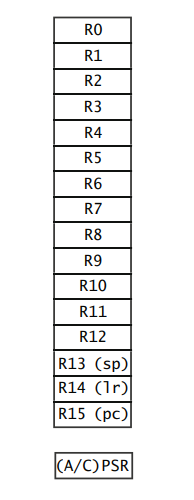
\includegraphics[width=3cm]{registersatz.PNG}
            \end{minipage}
            \begin{minipage}[t]{0.7\textwidth}
            \vspace{-2cm}
                \begin{itemize}
                    \item R0-R12: Normale Register 
                    \item R13-15: Spezialregister
                    \item R15: Program Counter 
                    \item (A/C) PSR TODO
                \end{itemize}
            \end{minipage}
    \end{itemize}
        
        

\end{document}